\documentclass[12pt]{article}

\usepackage{tikz}
\usepackage{geometry}
\usetikzlibrary{mindmap}

\pagestyle{empty}

\geometry{landscape, margin=1cm}

\begin{document}
\begin{center}
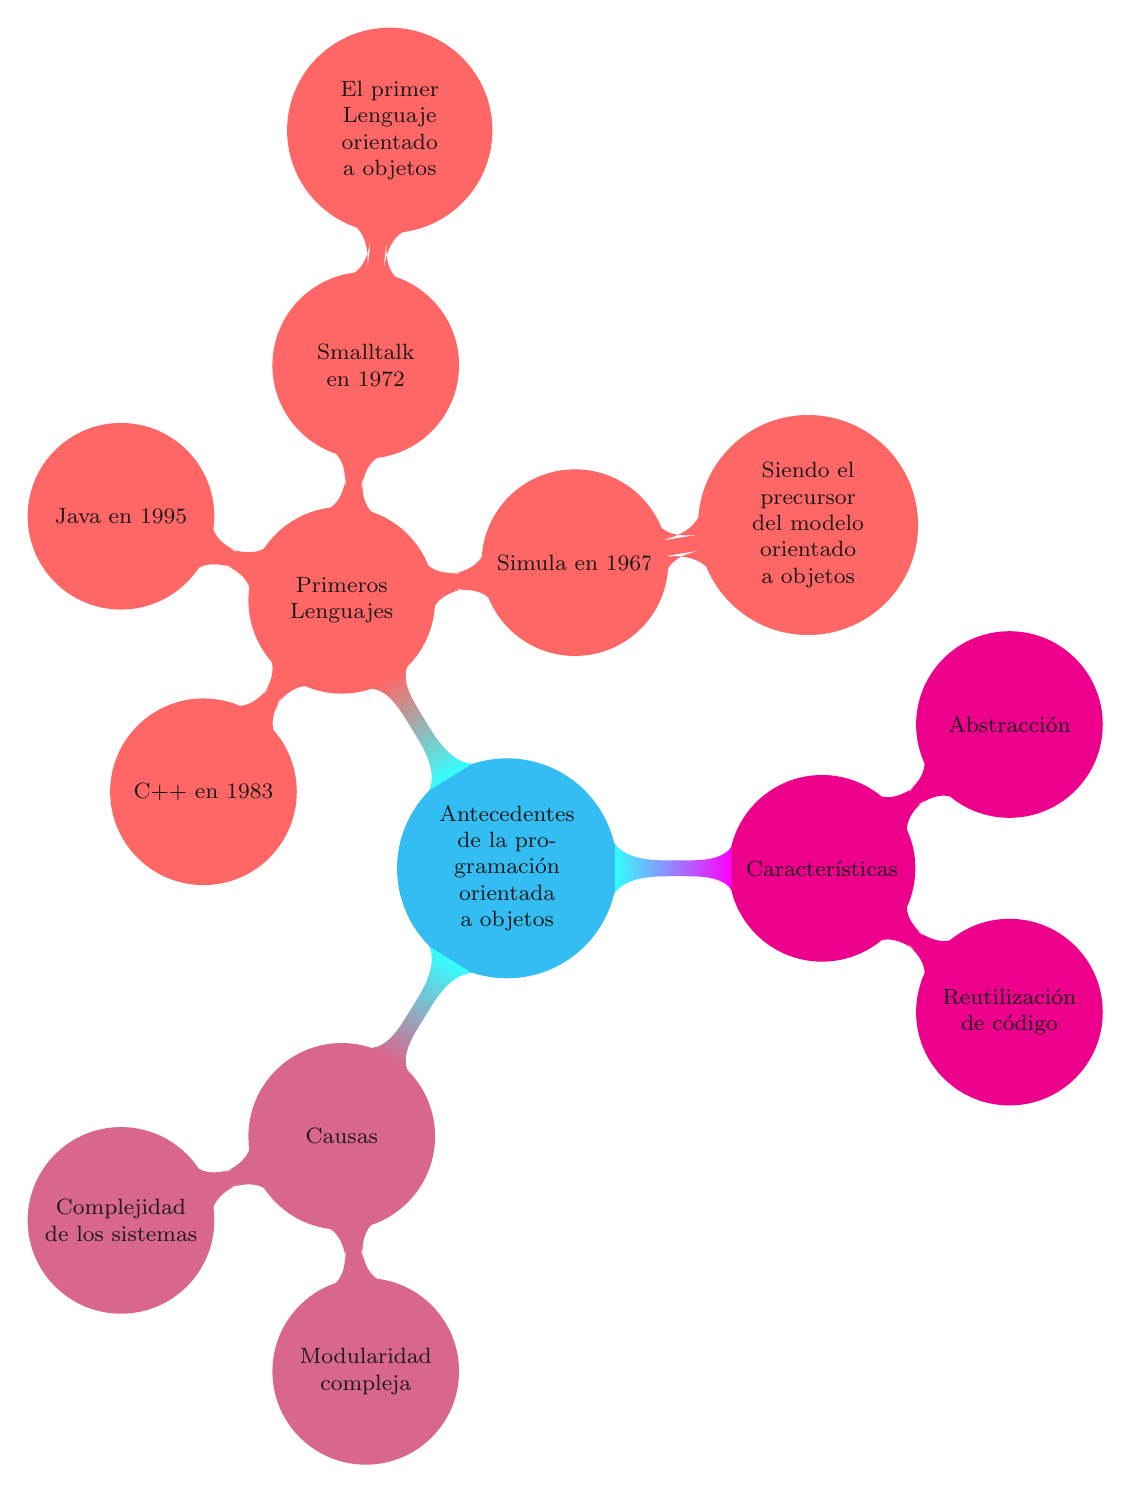
\begin{tikzpicture}[small mindmap, grow cyclic, every node/.style=concept, concept color=cyan!80, text=black!90,
        level 1/.style={level distance=4cm,sibling angle=365/3},
        level 2/.style={level distance=3cm,sibling angle=75},
        level 3/.style={level distance=3cm,sibling angle=20}]
    \node{Antecedentes de la programación orientada a objetos}
        child[concept color=purple!60] { node { Causas }
            child { node { Complejidad de los sistemas } }
            child { node { Modularidad compleja } }
        }
        child[concept color=magenta] { node { Características }
            child { node { Reutilización de código } }
            child { node { Abstracción } }
        }
        child[concept color=red!60] { node { Primeros Lenguajes }
            child { node { Simula en 1967 }
                child { node { Siendo el precursor del modelo orientado a objetos } }
            }
            child { node { Smalltalk en 1972 }
                child { node { El primer Lenguaje orientado a objetos } }
            }
            child { node { Java en 1995 } }
            child { node { C++ en 1983 } }
        }
    ;
\end{tikzpicture}
\end{center}
\end{document}
